\documentclass{emulateapj}
%\documentclass[12pt,preprint]{aastex}

\usepackage{graphicx}
\usepackage{float}
\usepackage{amsmath}
\usepackage{epsfig, floatflt}
\usepackage{natbib, hyperref}
\usepackage{url}
\usepackage{physics}

\begin{document}
	
	\title{Ast3310 Project Nr. 2: Modelling a Star}
	
	\author{Nils-Ole Stutzer}
	
	%\email{nilsole2009@live.no}
	
	%\altaffiltext{1}{Institute of Theoretical Astrophysics, University of
		%Oslo, P.O.\ Box 1029 Blindern, N-0315 Oslo, Norway}
	\section*{Introduction}
	In order to make a realistic model of a star one needs to include all (relevant) types of energy transport, transporting outwards the energy produced in the fusion reactions inside the stellar core. In the previous project we made a model of the radiative energy transport inside a star. However, we know that convection is the second important type of energy transport in a star, part form observations of the solar surface and part form previously done simulations. Thus, to improve our model of a star, we want to add convective energy transport to our already finished model of the radiative energy transport. 
	
	\section*{Method}
	In order to make a model of a realistic star we need to include an energy transport through convection in addition to the previously modelled radiative energy transport, as convection is the other dominant form of energy transport observed in stars. In the previous project we model a star by solving the coupled system of partal differential equations (PDEs) given by
	\begin{align}
		\pdv{r}{m} &= \frac{1}{4\pi r^2\rho}\\
		\pdv{P}{m} &= -\frac{Gm}{4\pi r^4}\\
		\pdv{L}{m} &= \epsilon\\
		\left(\pdv{T}{m}\right)_\text{stable} &= -\frac{3\kappa L}{256\pi^2\sigma r^4 T^3},
		\label{eq:proj1} 
	\end{align}
	by iterating inwards into the star over smaller and smaller mass shells using an Runge-Kutta Four (RK4) algorithm. Here $\rho$, m, L and $\epsilon$ denote the density, mass, luminosity
	and energy produced respectively per mass unit, within a shell of radius r and temperature T. In addition to these PDEs we assumed that the star consists of an ideal gas with constant mean molecular weight $\mu$ (using $X = 0.7$, $Y_\text{He-4} = 0.29$, $Y_\text{He-3} = 10^{-10}$, $Z = 0.01$, $Z_\text{Li-7} = 10^{-13}$ and $Z_\text{Be-7} = 10^{-13}$). Hence we can use the equation of state for an ideal gas to determine the pressure.
	
	In addition to the above given PDEs we need a PDE representing the total temperature gradient, so as to include a convective temperature gradient. The total temperature gradient $\pdv{T}{m}$ depends on whether radiation or convection is the dominant energy transportation. Thus, we need to determine when each energy transport type is dominant, so as to adapt the temperature gradient accordingly. If the radiative energy transport is unable to transport all energy, convection will start. Also for convection to happen, a rising blob of gas must have a higher temperature than its surrounding. Then a blob becomes buoyant. If in addition the mean free path of a photon is much smaller then the blobs size excess energy in the blob (due to heat) doesn't leave the blob too fast via radiation. To find out whether there is convection we can use the inequality given by the instability criterion for convection
	\begin{align}
		\nabla_\text{stable} > \nabla^*>\nabla_p>\nabla_\text{ad},
	\end{align}
	which include all the above mentioned criteria. Here $\nabla_\text{stable}$ is the radiative temperature gradient, $\nabla^*$ is the stars temperature gradient, $\nabla_p$ is the temperature gradient of a rising gas blob and $\nabla_\text{ad}$ is the adiabatic temperature gradient. All the $\nabla$s are defined as $\nabla_i = \left(\pdv{\ln(T)}{\ln(P)}\right)_i = -\frac{H_P}{T}\left(\pdv{T}{r}\right)_i$, where the index $i$ stand for the different types of thermodynamic processes (like "stable", "*", etc.). We also know that the total energy flux $F$ is simply the sum of the radiative and convective energy flux $F_R$ and $F_C$ we get that
	\begin{align}
		F_R + F_C = \frac{16\sigma T^4}{3\kappa\rho H_P}\nabla_\text{stable} = \frac{L}{4\pi r^2},
		\label{eq:flux}
	\end{align} 
	for the Stefan-Boltzmann constant $\sigma$, the temperature $T$, density $\rho$, opacity $\kappa$, the pressure scale height $H_P$, luminosity $L$ and radius $r$ of a shell in the star. 
	We find the pressure scale height by assuming a static atmosphere, where gravity and pressure forces are the only present forces. From the 1D equation of motion we find that
	\begin{align}
		\rho\left(\pdv{}{t} + v\pdv{}{r}\right)v = -\nabla P + F = 0,
	\end{align}
	for since the atmosphere is assumed to be static. Hence the pressure gradient
	\begin{align}
		\nabla P = F = -g\rho \implies \pdv{P}{r} = -g\rho,
	\end{align}
	for a gravitational field strength $g = G\frac{m}{r^2}$. Using the definition of the pressure scale height $H_P \equiv -P \pdv{r}{P}$ we get an expression $H_P = \frac{P}{\rho g} = \frac{k_B T}{g\mu m_u}$, for an ideal gas. Here $k_B$ is the Boltzmann constant, $m_u$ is one atomic mass unit in kg, $\mu$ is the mean molecular weight.
	We also assume that the scale height $H_P = l_m/\gamma$, where $l_m$ is the mixing length of a gas blob and $\gamma=1$ is some parameter.
	
	Using the last equality in eq. (\ref{eq:flux}) to solve for $\nabla_\text{stable}$, needed to test whether the instability criterion is fulfilled, and get 
	\begin{align}
		\nabla_\text{stable} = \frac{3\kappa\rho H_P L}{64\pi r^2\sigma T^4}.
	\end{align}
	Since we have also assumed that the star consists of an ideal gas we can find the adiabatic temperature gradient defined as 
	\begin{align}
		\nabla_\text{ad} = \left(\pdv{\ln(T)}{\ln(P)}\right)_\text{ad} = \frac{P\delta}{T\rho c_P},
	\end{align}	
	where $c_P$ is the specific heat capacity at constant pressure, and $\delta = -\left(\frac{\ln(\rho)}{\ln(T)}\right)_P = \frac{T}{V}\left(\pdv{V}{T}\right)_P = 1$ for an ideal gas. The specific heat capacity at constant pressure is found from 
	\begin{align*}
		c_P - c_V = nk_B,
	\end{align*}
	for an ideal gas. Then inserting $c_V = \left(\pdv{u}{T}\right)_V = \frac{3}{2}\frac{n}{k_B}$ we get that $c_P = \frac{5}{2}n k_B = \frac{5}{2}\frac{k_B}{m_u\mu}$, where $n$ is the specific number density of gas particles and $u$ is the specific internal energy of the gas. 
	Thus, the adiabatic temperature gradient for an ideal gas is simply $\nabla_\text{ad} =\frac{2}{5}$.  We can now use the condition $\nabla_\text{stable}>\nabla_\text{ad}$ as an instability criterion, so as to determine if we have convection or not. If it is fulfilled we get a convectively unstable gas resulting in convection, making it necessary to update the temperature gradient to the convective one. While if the condition is not satisfied the temperature gradient is simply the one found in a radiative zone (the one we used in the first project, eq. (\ref{eq:proj1}). 
	
	In case of convection the actual total temperature gradient $\nabla^*$ includes both radiation and convection, since energy can be transported by both convection and radiation in case of convection. Therewhile, if there is no convection all energy is transported by radiation making the actual temperature gradient $\nabla^* = \nabla_\text{stable}$.  
	
	If we consider the case where there is convection we can use that $F_R = \frac{16\sigma T^4}{3\kappa\rho H_P}\nabla^*$ we can solve eq. (\ref{eq:flux}) for $\nabla^*$ to find the convective temperature gradient. Using the definition of the $\nabla$s we find the convective temperature gradient in terms of derivatives by 
	\begin{align}
		\nabla^* &= -\frac{H_P}{T}\pdv{T}{r} = -\frac{H_P}{T}\pdv{T}{m}\pdv{m}{r} = -4\pi r^2\rho\frac{H_P}{T}\pdv{T}{m}\\
		&\implies \left(\pdv{T}{m}\right)_\text{conv} =- \frac{T}{4\pi r^2 \rho H_P}\nabla^*
	\end{align}
	In order to calculate $\left(\pdv{T}{m}\right)_\text{conv}$ we must first find an equation for $\nabla^*$.
	To do that we again take a look at eq. (\ref{eq:flux}), and solve it for $\nabla^*$, which in case of convectively unstable gas is the convective temperature gradient.
	We see that we need an expression for the convective energy flux $F_C$ in order to solve eq. (\ref{eq:flux}) for $\nabla^*$. If we now insert the expression for the convective energy flux
	\begin{align}
		F_C = \rho c_P T\sqrt{g\delta} H_P^{-3/2}\left(\frac{l_m}{2}\right)^2(\nabla^* - \nabla_p)^{3/2}
	\end{align}
	(note that $F_C=0$ if there is no convection) in addition to the expression $F_R = \frac{16\sigma T^4}{3\kappa\rho H_P}\nabla^*$ into eq. (\ref{eq:flux}) we can find an expression for $\xi^2\equiv(\nabla^*-\nabla_p)$:
	\begin{align*}
		F_R + F_C &= \frac{16\sigma T^4}{3\kappa\rho H_P}\nabla^* \\
		&+ \rho c_P T\sqrt{g\delta} H_P^{-3/2}\left(\frac{l_m}{2}\right)^2(\nabla^* - \nabla_p)^{3/2} \\
		&= \frac{16\sigma T^4}{3\kappa\rho H_P}\nabla_\text{stable}\\
		\implies \xi^3&=\left(\nabla^* - \nabla_p\right)^{3/2} = \frac{64\sigma T^3\sqrt{H_P}}{3\kappa\sqrt{\delta}c_P l_m^2\rho^2\sqrt{g}}\left(\nabla_\text{stable}-\nabla^*\right).
	\end{align*}
	If we then let $U \equiv \frac{64\sigma T^3}{3\kappa\rho^2c_P}\sqrt{\frac{H_P}{g\delta}}$, we can write 
	\begin{align}
		\xi^2 = (\nabla^*-\nabla_p) = \left(\frac{U}{l_m^2}(\nabla_\text{stable} - \nabla^*)\right)^{2/3}.
		\label{eq:XiThirdDeg1}
	\end{align}
	Then we also need the relation
	\begin{align}
		(\nabla_p - \nabla_\text{ad}) = (\nabla^* - \nabla_\text{ad}) - (\nabla^* - \nabla_\text{ad})
		\label{eq:nablarelation}
	\end{align}
	as well as 
	\begin{align}
		(\nabla_p - \nabla_\text{ad}) = \frac{32\sigma T^3}{3\kappa \rho^2 c_P v}\frac{S}{Qd}(\nabla^* - \nabla_p),
		\label{eq:blobwork}
	\end{align}
	where $S$ is the surface of a rising gas blob, $Q$ is the area of the blob that is perpendicular to the blobs rising speed $v$ and $d$ is the blob's diameter. The speed the blob rises with is given by 
	\begin{align}
		v = \sqrt{\frac{g\delta l_m^2}{4H_P}}\xi.
		\label{eq:blobspeed}
	\end{align}
	We can now find a second order equation for $\xi$ by inserting eq. (\ref{eq:blobwork}) and (\ref{eq:blobspeed}) into eq. (\ref{eq:nablarelation}). We then find that 
	\begin{align}
		&\frac{32\sigma T^3}{3\kappa\rho^2c_P}\sqrt{\frac{4 H_P}{g\delta l_m^2}}\xi^{-1} \frac{S}{Qd}\xi^2 = (\nabla^* - \nabla_\text{ad}) - \xi^2\\
		&\implies \frac{U\Gamma}{l_m}\xi = (\nabla^* - \nabla_\text{ad}) - \xi^2,
	\end{align}
	for the geometric factor $\Gamma \equiv \frac{S}{Qd}$. The resulting second order equation
	\begin{align}
		\xi^2 + \frac{U\Gamma}{l_m}\xi + (\nabla_\text{ad} - \nabla^*) = 0
	\end{align}
	has two solutions
	\begin{align}
		\xi = -\frac{U\Gamma}{2l_m}\pm \frac{1}{2}\sqrt{\frac{U^2\Gamma^2}{l_m^2} + 4(\nabla^* - \nabla_\text{ad})}.
	\end{align}
	But since $\xi>0$ we want a positive solution. This only happens for the "$+$" solution as 
	$\frac{1}{2}\sqrt{\frac{U^2\Gamma^2}{l_m^2} + 4(\nabla^* - \nabla_\text{ad})}>\frac{U\Gamma}{2l_m}$, because the instability criterion states that $\nabla^* > \nabla_\text{ad}$. The only viable solution is therefore 
	\begin{align}
		\xi = -\frac{U\Gamma}{2l_m^2} + \frac{1}{2}\sqrt{\frac{U^2\Gamma^2}{l_m^2} + 4(\nabla^* - \nabla_\text{ad})}.
	\end{align}
	Solving this newly obtained solution for $\nabla^*$ we find $\nabla^* = \xi^2 + \frac{U\Gamma}{l_m}\xi + \nabla_\text{ad}$. By inserting this into eq. (\ref{eq:XiThirdDeg1}) we can eliminate the dependence on $\nabla^*$:
	\begin{align*}
	 	\xi^3 &= \frac{U\Gamma}{l_m^2}(\nabla_\text{stable} - \nabla^*) = \frac{U\Gamma}{l_m^2}(\nabla_\text{stable} - \xi^2 - \frac{U\Gamma}{l_m}\xi - \nabla_\text{ad})\\
	 	&\implies \xi^3 + \frac{U}{l_m^2}\xi^2 + \frac{U^2\Gamma}{l_m^3}\xi + \frac{U}{l_m^2}(\nabla_\text{ad} - \nabla_\text{stable}) = 0.
	\end{align*}
	We now consider the geometric factor $\Gamma$. If we assume that the gas blobs are spherical and rise straight upwards in case of convection, we let the surface of the blob $S = 4\pi r_P^2$ and the area perpendicular to the rising direction $Q = \pi r_p^2$, for the blobs radius $r_p = d/2$. Furthermore we assume that the mixing length $l_m = 2r_p$ so that we can write $\Gamma = \frac{S}{Qd} = \frac{4\pi r_p^2}{\pi r_p^2 2r_p} = \frac{2}{r_p} = \frac{4}{l_m}$. Inserting the expression for the geometric factor into the third order equation for $\xi$ we get
	\begin{align}
		\xi^3 + \frac{U}{l_m^2}\xi^2 + \frac{4U^2}{l_m^4}\xi + \frac{U}{l_m^2}(\nabla_\text{ad} - \nabla_\text{stable}) = 0,
		\label{eq:thirddeg}
	\end{align}
	which now only depends on known quantities. This third degree equation is then solved numerically for each step in the integration loop. Equation (\ref{eq:thirddeg}) should always have one real root, which is the one used to find the temperature gradient. If there are more than two complex roots, the program prints out a warning.
	As described earlier the new temperature gradient is found by fist solving eq. (\ref{fig:flux}) for $\nabla^*$, giving 
	\begin{align}
		\nabla^* &= \frac{3\kappa\rho H_P}{16\sigma T^4}\left(\frac{L}{4\pi r^2} - F_C\right)\\
		&= \frac{3\kappa\rho H_P}{16\sigma T^4}\left(\frac{L}{4\pi r^2} - \rho c_P T\sqrt{g\delta} H_P^{-3/2}\left(\frac{l_m}{2}\right)^2\xi^{3}\right),
	\end{align}
	then from the definition $\nabla^* $ we find the convective temperature gradient
	\begin{align}
		&\left(\pdv{T}{m}\right)_\text{conv} =\nonumber\\
		&- \frac{3\kappa}{64\pi r^2\sigma T^3 }\left(\frac{L}{4\pi r^2} - \rho c_P T\sqrt{g\delta} H_P^{-3/2}\left(\frac{l_m}{2}\right)^2\xi^{3}\right)\nonumber.
	\end{align}
	
	The function that previously returning the derivatives used to solve the four coupled non-linear partial differential equations (PDEs), is overwritten to include the above mentioned test whether there is convection or not. The temperature gradient is then updated accordingly, so that 
	\begin{align}
		\pdv{T}{m} =
		\begin{cases}
			\left(\pdv{T}{m}\right)_\text{rad}&\text{,if } \nabla_\text{stable}<\nabla_\text{ad}\\
			\left(\pdv{T}{m}\right)_\text{conv}&\text{,if } \nabla_\text{stable}>\nabla_\text{ad}
		\end{cases}
	\end{align}
	
	When having made a stable simulator (meaning having passed all sanity checks), we can move on to the main goal of this project, being that we want to make a model of a star where $L$, $m$ and $r$ are all going to zero within $\pm$5\% of $L_0$, $M_0$ and $R_0$. Also we want a stellar core reaching out at least 10\% of the initial radius, and we want a continous convection zone near the stellar surface that should be at least 15\% of $R_0$. If possible there shouldn't be any convection in the stars core, or at least as thin as possible with a small convective flux. Last we also want a model where the PPI chain dominates at low $T$, while having PPII and PPIII dominate at hight $T$. 
	
	To find the best model of a star we can then change each initial parameter, while holding the others constant, or combining changes to see how they affect the model. The default initial values will be $L_0 = L_\odot$, $R_0 = R_\odot$, $M_0 = M_\odot$, $\rho_0 = 1.42\cdot 10^{-7}\overline{\rho}_\odot$, $T_0 = 5770$ K, being the approximate surface parameters of the sun. We allow a change to the initial parameters $R_0$, $\rho_0$ and $T_0$ between a factor 0.2 to 5. Changes to the initial density, however, we allow arbitrarily hight or low. Then following the tendencies found by changing initial parameters, we may find a model which satisfies our goals. 
	
	\section*{Results/Discussion}
	Each time finishing a part of the program modelling the star, we compared the programs output to a provided sanity check. Generally each sanity check was passed, without any significant problems. In the first sanity check, where we compared the program output for a row of given input parameters, there was a small deviation form the wanted output parameters. This however, was somewhat expected as it is possible to find a convective temperature gradient in slightly different ways, each resulting in somewhat differently rounded off results. Because the resulting outputs were in the right order of magnitude and the round-off errors did not deviate significantly we concluded that the first sanity check was passed. When comparing provided sanity check plots to the ones the program produced, we found no visible difference, concluding that also this was a successfully passed sanity check.
	
	\begin{figure*}
		\centering
		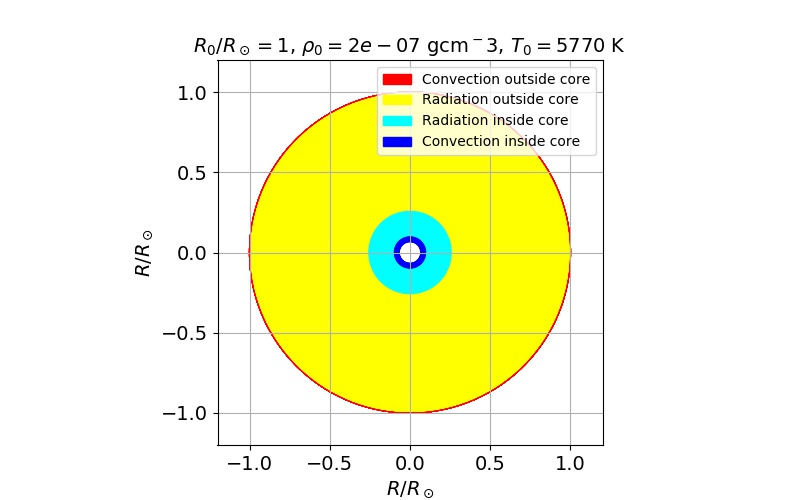
\includegraphics[width=1\columnwidth]{CrossSec1.jpg}
		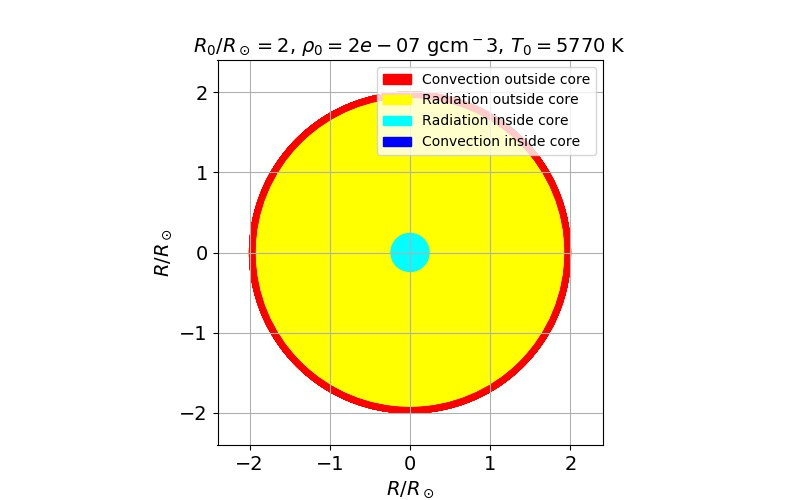
\includegraphics[width=1\columnwidth]{CrossSec2.jpg}
		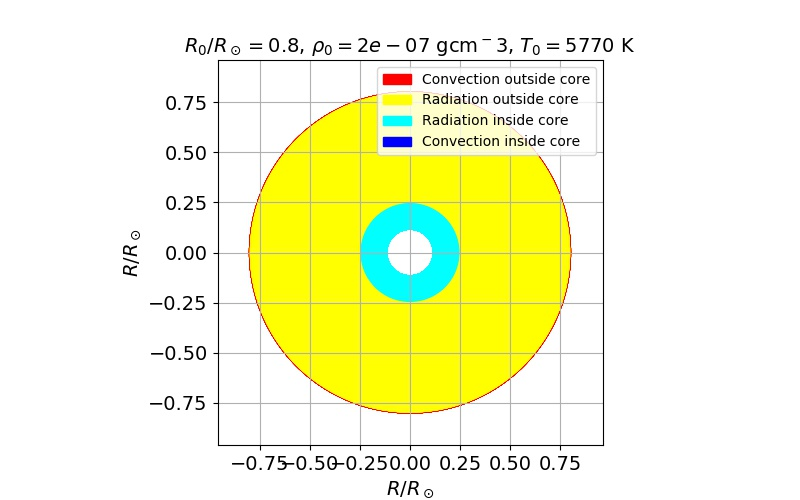
\includegraphics[width=1\columnwidth]{CrossSec3.jpg}
		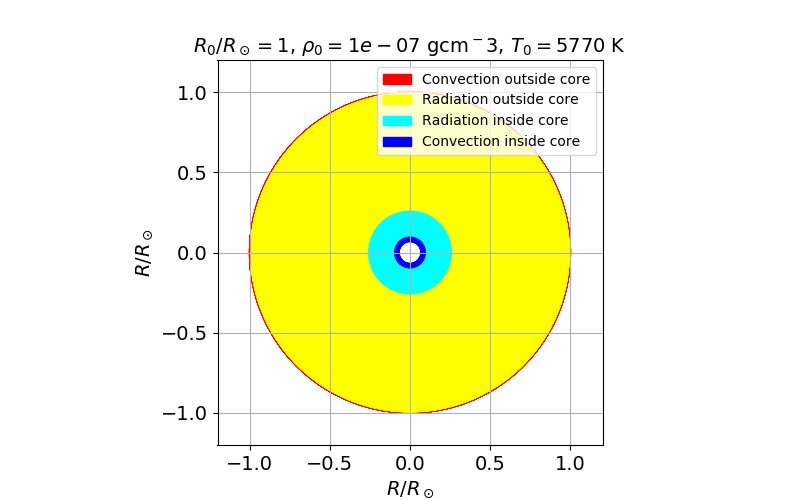
\includegraphics[width=1\columnwidth]{CrossSec4.jpg}
		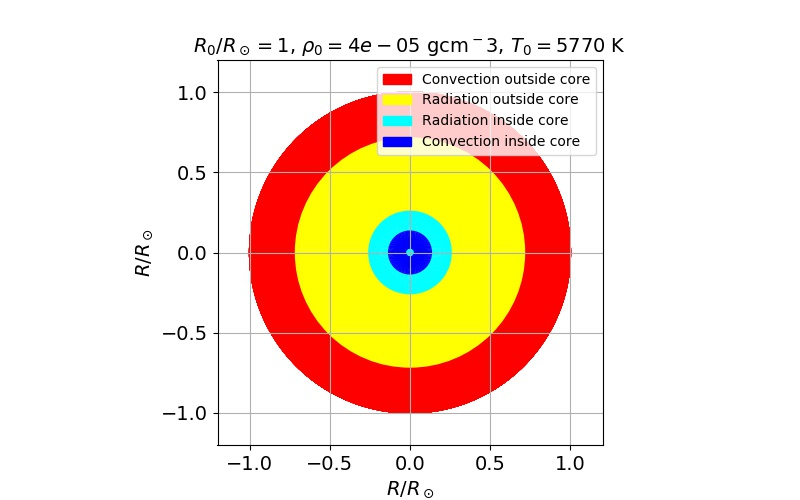
\includegraphics[width=1\columnwidth]{CrossSec5.jpg}
		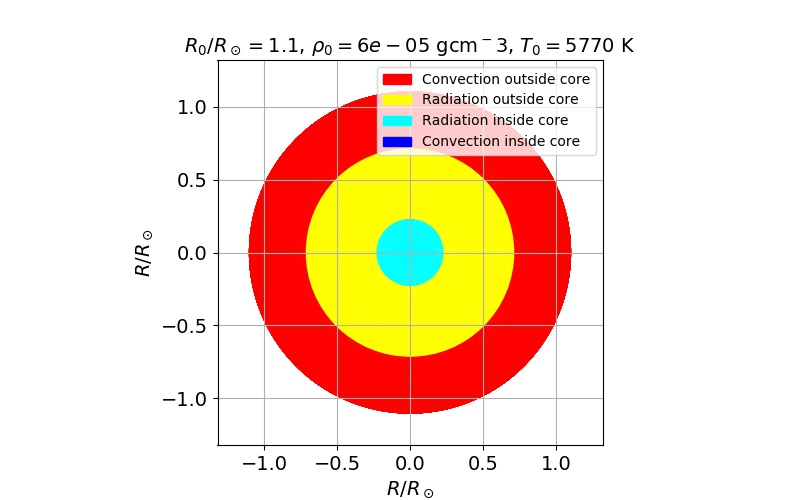
\includegraphics[width=1\columnwidth]{CrossSec6.jpg}
		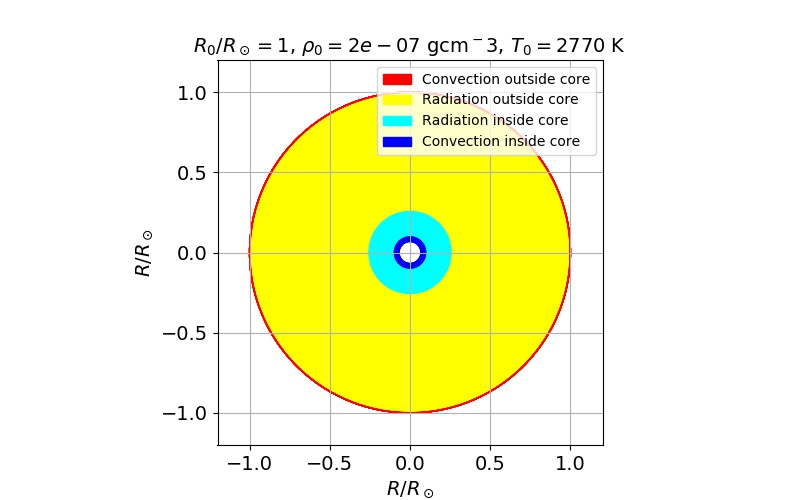
\includegraphics[width=1\columnwidth]{CrossSec7.jpg}
		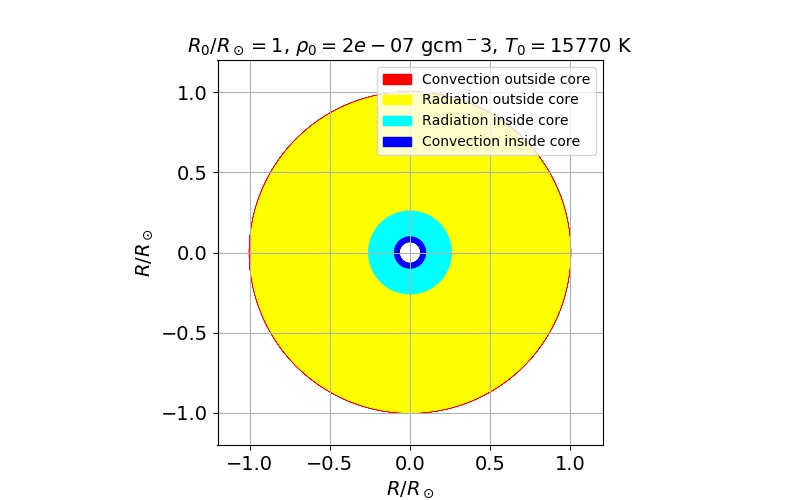
\includegraphics[width=1\columnwidth]{CrossSec8.jpg}
		\caption{The figure shows eight plots of stellar cross-sections using different initial radii $R_0$, initial densities $\rho_0$ and initial temperatures $T_0$. The choices of initial parameters are shown above each plot. Whether a layer is radiation or convection dominated is indicated by colour code.}
		\label{fig:CrossSec}		
	\end{figure*}
	
	We found that using an accuracy of $p = 0.01$ in the variable step length, assuring a local error in the RK4 algorithm less than $10^{-2}$, produced a satisfactory result.
	
	When experimenting with different choices of initial values for the radius $R_0$, density $\rho$ and temperature $T_0$ (we excluded the pressure $P_0$ as it is determined by the density and the temperature through the equation of state) we found that it was much easier to find a model fulfilling the goals, than in the previous project that only included the radiative energy transport. That may have something to do with the fact that a radiation dominated star is not that realistic (or at least uncommon), as most stars have a combination of radiative and convective energy transport. Thus if the radiative energy transport becomes ineffective, the convection might take over (or vice versa), producing a more effective energy transport over all. This seems to make the overall model more stable and thus easier to work with. 
	
	The cross-sections of the stars produced by our model can be seen in Fig. \ref{fig:CrossSec}. Each individual cross-section is produced by different choices of initial parameters (which are shown above each individual plot). The first cross-section in the first row in Fig. \ref{fig:CrossSec} shows the star produced when using the default initial radius $R_0 = R_\odot$, density $\rho_0 = 1.42\cdot 10^{-7}\overline{\rho}_\odot$ and temperature $T_0 = 5770$ K (this corresponds to the sanity check cross-section). We see that it has a quite thin convection zone at its surface and a relatively thin convection zone in the stellar core. Most of its cross-section is dominated by a radiative zone extending from the core and almost to the surface. Note also that the relatively large white spot in the stars centre, characterizes a model where the integration loop stopped to early, not finishing close enough to the stars centre.
	
	Next, when letting the temperature and density stay default, but let the initial radius $R_= = 2R_\odot$ we see that the convection zone at the surface increased in thickness (see right toppmost in Fig. \ref{fig:CrossSec}). The radiation zone now stretches from the very centre to the outer convection zone, this time not having a convection zone in the core. Also this time the integration was not stopped to early.
	
	When letting the initial radius $R_0 = 0.8 R_\odot$ we see that the opposite effect is seen as when increasing the initial radius (see second row left in Fig. \ref{fig:CrossSec}). Again the outer convection zone is virtually non-existent, having a almost exclusively radiation dominated star. However, similarly as seen in the first cross-section, the integration stopped prematurely as indicated by the white spot in the stars centre. It seems as if a larger initial radius is needed in order to achieve a thicker outer convection zone.
	
	Decreasing the initial density by half of the default, while letting the other initial parameters be their default, seems to have a similar effect to decreasing the initial radius (see second row right in Fig. \ref{fig:CrossSec}). The outer convection zone in this case, is as for the low initial radius, virtually non-existent. Again most of the stars cross-section is dominated by radiative energy transport, this time however, also having a small convection zone in the very core. The integration loop seems to have stopped too early in this case also.
	
	Now increasing the initial density by a factor of 200 (remember we permit arbitrarily high changes $\rho_0$), while not changing the other initial parameters, we observe a significantly thicker convection zone near the stars surface (see third row left in Fig. \ref{fig:CrossSec}). The radiation zone in this case stretches all the way from the outer convection zone and well into the core. In the very centre of the core there is a small radiative zone, surrounded by a quite thick convective zone inside the core. We therefore conclude that a significant increase of the initial density seems to be needed for a satisfactory outer convection zone. 
	
	Since we observed that larger initial radii and densities where needed for a thicker outer convection zone, as well as an integration that didn't stop prematurely, we tried to increase both the initial radius and density to $R_0 = 1.1 R_\odot$ and $\rho_0 = 6\cdot10^{-5}$ gcm$^{-3}$ (see third row right in Fig. \ref{fig:CrossSec}). This time we obtained a star with a thick (continuous) outer convection zone, as well as having no convection zone at all in the core. The obtained model seems to be the best one so fare, as it at first glance already has fulfilled the goals. 
	
	For consistency we also tried to only change the initial temperature, while leaving the other initial parameters as their default (see the two bottommost plots in Fig. \ref{fig:CrossSec}). However, changing the initial temperature upwards or downwards did not seem to have any significant effect. The models essentially look identical to the one where no initial parameter changes where made. Thus it seems as if changing the temperature doesn't change the model that much. However, more experimenting is needed to say this for sure. 
	
	We conclude that combining an increased initial radius and a quite significantly increased initial density results in a thick outer convection zone, while leaving the rest of the star consist of a radiation zone with a core that is not too small. Also the integration is essentially completed into the very core. If we take a look at the instability criterion $\nabla_\text{stable}>\nabla_\text{ad}$ and insert the definition of $\nabla_\text{stable}$ as well as $\nabla_\text{ad}= 2/5$ for an ideal gas. Then we get $-\frac{4\pi r^4 \rho k_B}{Gm\mu m_u}\left(\pdv{T}{m}\right)_\text{stable} > 2/5$, utilizing the definition of the scale height $H_P$ as well as gravitational field strength $g$. We see that indeed the instability criterion tells the same story as the cross-section plots in Fig. \ref{fig:CrossSec}. We see that since $\left(\pdv{T}{m}\right)_\text{stable}$ is negative $\nabla_\text{stable}$ is positive. Furthermore, we see that $\nabla_\text{stable}\propto r^4$ and also $\nabla_\text{stable}\propto\rho$, but $\nabla_\text{stable}$ is only implicitly dependent on the temperature $T$. Thus a relatively small positive change in the radius will make $\nabla_\text{stable}$ increase quite a lot, while we have to change the density $\rho$ by a lot in order to change $\nabla_\text{stable}$ a lot. So just as seen in the plots of the cross-sections in Fig. \ref{fig:CrossSec} we see that we need a small positive change in the initial radius and a quite dramatic positive change in the initial density in order to get deep convection zones. But of course there is a trade-off, in the sense that one can get extremely deep convection zones by increasing both $R_0$ and $\rho_0$ by a lot, but end up with other features that seem unphysical (like too small cores or that the integration does not go to the very centre of the star). When it comes to the temperature $T$, we see that an factor 0.2 to 5 change to $T_0 = 5770$ K, will still be quite a small compares to the temperatures further into the star (in the MK range). As the temperature only affects $\nabla_\text{stable}$ implicitly through $\left(\pdv{T}{m}\right)_\text{stable}$ and since the surface temperatures we can choose are quite small, they don't affect the stability criterion at the surface that much, rendering the initial temperature somewhat uninteresting.
	
	However, the instability criterion only states when there is convection, not how broad a convection zone will be. To find out how to obtain a deep convection zone from analytical expressions is difficult since all relations involved are coupled and non-linear. Nevertheless, we may obtain an initial understanding of how to start up with a big $\nabla_\text{stable}$, from the discussion in the previous paragraph, and thus how to start of with a convection zone at the outer regions of the star. Also when staring of with a big $\nabla_\text{stable}$, the layer may remain convective for longer when going inwards, as it $\nabla_\text{stable}$ has to drop of dramatically before the instability is broken. Therefore determining the depth of a convection zone is done numerically in our case.
	
	Anyway, it seems as if initial value choices of $R_0=1.1R_\odot$, $\rho_0 = 6\cdot 10^{-5}$gcm$^{-3}$ and $T_0 = 5770$K are a good ones. Since it combines a slight increase in the initial radius, a quite dramatic increase in the initial density and no change in initial temperature, the model will start of with a convection zone at the surface. But also we see from the cross-section that the convection zone is indeed quite deep, while the other structures look quite good too. 
	
	\begin{figure*}
		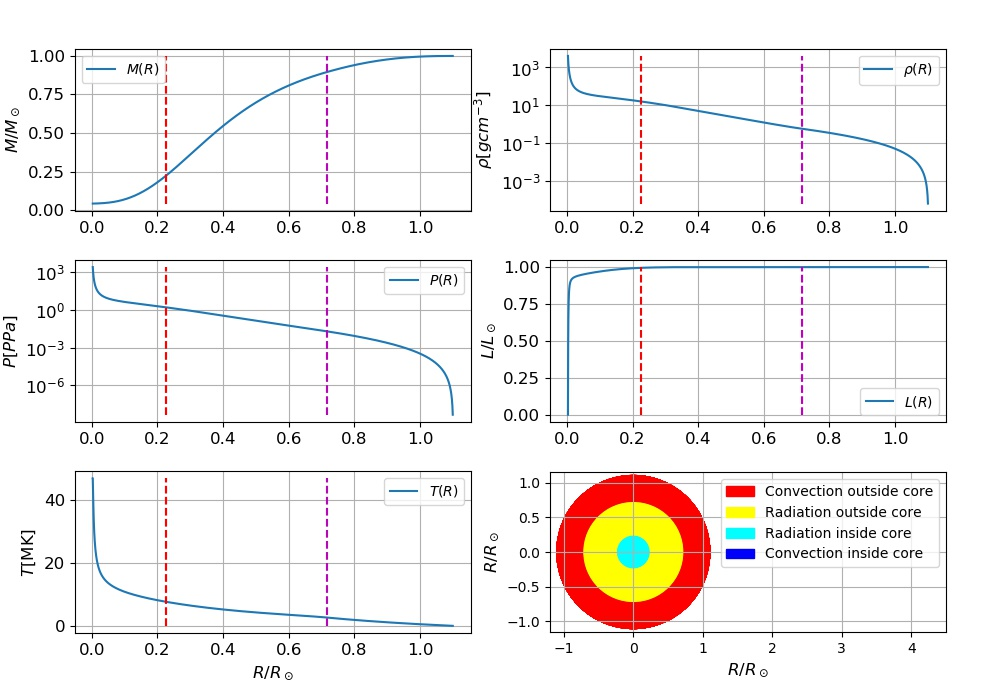
\includegraphics[width=\textwidth]{modelbest.jpg}
		\caption{The figure shows plots of the mass $M$, the density $\rho$, pressure $P$, luminosity $L$ and temperature $T$ as functions of the radial distance $R$ from the core of the best model found. Also a cross-section of the best model found is included in the lower right. The core and outer convection zone radii are indicated by dotted red and magenta lines respectively.}
		\label{fig:modelbest}
	\end{figure*}
	
	We now take a more detailed look at the so far best model (see third row to the right in Fig. \ref{fig:CrossSec}). In Fig. \ref{fig:modelbest} one can see the mass $M(r)$, the density $\rho(R)$, the pressure $P(R)$, the luminosity $L(R)$, the temperature $T(R)$ and the cross-section of the model, all as functions of the radial distance $R$ from the centre of the star. It turns out that the radial distance $R$, the mass $M$ and the luminosity $L$ all approach zero within the $\pm$5\% tolerance or their respective initial values. The radial distance approaches zero within 0.3\% of its initial value $1.1R_\odot$. The mass approaches zero within about $4.2$\% of the initial value of $M_\odot$, while the luminosity went all the way down to zero. The first part of the goals are thus reached.
	
	\begin{figure*}
		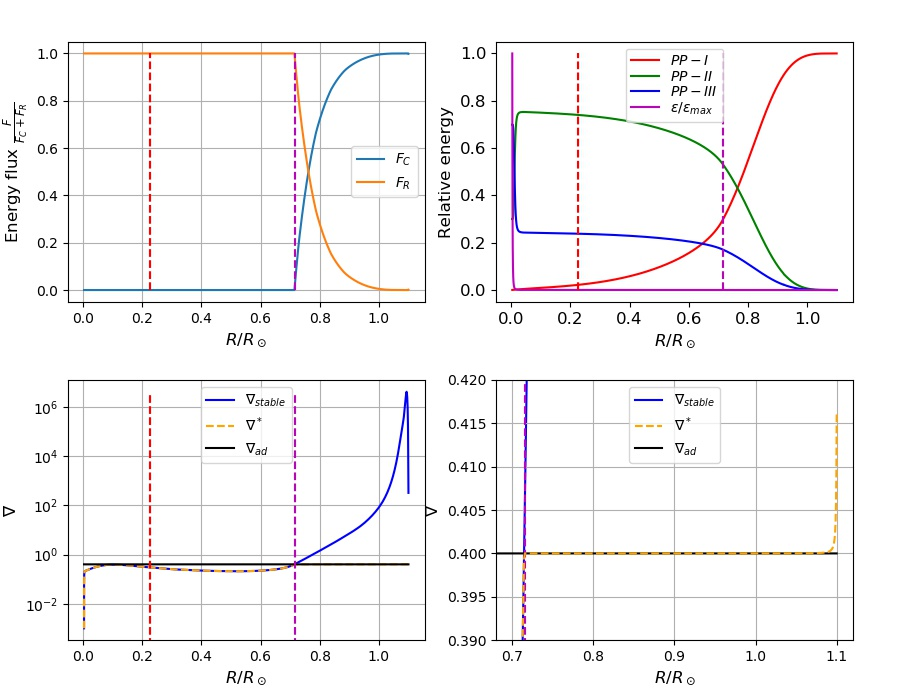
\includegraphics[width=\textwidth]{fluxplot.jpg}
		\caption{The figure shows a plot of the normalized convective energy flux $F_C$ and the radiative energy flux $F_R$ (upper left). In the upper right the relative energy production for each PP-chain as well as the energy production $\epsilon$ are shown. The two bottom plots are the temperature gradients ($\nabla$s), where the rightmost is an enlargement of the leftmost plot at the outer convection zone. The core and outer convection zone radii are indicated by dotted red and magenta lines respectively.}
		\label{fig:flux}
	\end{figure*}
	
	When looking at the mass distribution $M(R)$ (see Fig. \ref{fig:modelbest}) over the stars cross-section we see that the mass props gradually when going inwards. The relatively slow decrease in the outer layers indicates a relatively low mass density making the mass derivative small. Going further inwards we see that the mass drops faster and faster when going thought the stars radiation zone, indicating an increasing density, before the slope again decreases when crossing into the very core of the star. The slope of the mass distribution in the very core decreases even though the density sky-rockets, which is due to the small radius dominating the mass gradient as $\pdv{m}{r}\propto r^2$ is parabola-like for small radii.
	
	Looking at the density $\rho(R)$ and pressure $P(R)$ distributions in Fig. \ref{fig:modelbest}, we see that they behave very similar over the stars cross-section. This is no surprise as the two quantities are tightly couples through the equation of state of an ideal gas. In the outer regions of the star both $\rho$ and $P$ start of really low, but with a steep slope. After increasing sharply over a small negative radius change, the slope changes to a somewhat linear fashion. This tendency continues until the very core of the star, where both quantities start to sky-rocket upwards, as the enormous mass from the rest of the star pushes inwards on the core due to gravity. 
	
	The temperature over the cross-section in Fig. \ref{fig:modelbest} starts of quite low, and with a shallow slope. As moving inwards through the convection zone the temperature really only increases marginally. This tendency continues when going though the radiation zone outside the core. But when approaching the core, the temperature starts to curve upwards more and more, before suddenly increasing exponentially in the very core of the star. 
	
	Finally we see that the luminosity over the stars cross-section in Fig. \ref{fig:modelbest} is almost constantly equal to $L_\odot$ over most of the stars cross-section. This is expected, as a star almost exclusively produces its energy inside its core. In the core region we see that the luminosity drops faster and faster, before suddenly falling of to zero over a very short radius interval in the very core. This is also expected behaviour, since the amount of fusionable material inside ever decreasing shells when integrating inwards resulting in a sharp decrease in energy production and thus luminosity.
	
	All in all we can conclude that the mass $M(r)$, the density $\rho(R)$, the pressure $P(R)$, the luminosity $L(R)$, the temperature $T(R)$ are all behaving according to known theory, indicating a so far successful model of a star.
	
	Now we take a look at the layers of the cross-section of the best model. The core, meaning the region where $L/L_\odot < 0.995$, extends about to a radial distance of $R_c \approx 0.23R_\odot$, which corresponds to about 21\% of its initial radius. According to \cite{Garcia:2007} and \cite{Davis:2016} the Sun's core is between $0.2R_\odot$ and $0.25R_\odot$, so in other words around 20-25\% of the Sun's radius. The core radius in our model, being about $R_c = 0.23R_\odot$ or 21\% of the initial radius, falls right into this interval. The outer (continuous) convection zone extends from about $R_\text{conv} \approx 0.716 R_\odot$ to $R_0 = 1.1R_\odot$, corresponding to a thickness of 35\% of the initial radius $R_0$. Compared to the Sun's convection zone, which according to \cite{Dalsgaard:1991} and \cite{Basu:1997} is estimated to have a depth of $(0.287 \pm 0.003)R_\odot$ and an inner radius of $(0.713 \pm 0_001)R_\odot$, we see that the convection zone in our model is a little thicker. The radiation zone (outside of the core) in our model has a thickness of about $0.49R_\odot$ or around $44$\% of the initial radius. In the Sun the radiation zone (outside of the core) is quite comparable, although a bit thicker, having about a depth of about $0.5R_\odot$. It appears as if the best model star we have found is quite similar to the Sun, only differing somewhat in the thickness of the different cross-section structures.
	
	We notice that most experimental estimates will have an associated uncertainty. That is partly due to uncertainties in the measurements, but may also be due to that the Sun's shell like structures are not shaped like perfect spheres, but rather egg or ellipsoid shaped due to its rotation. Thus different parts along the same shell-like structurein the Sun have different radii. As we have not included the rotation of the star in our model, every point along a spherical shell will exhibit the same properties, meaning the core, radiation and convection zones are all perfectly spherical. 
	
	In Fig. \ref{fig:flux} one can see four plots. The top-left one shows a plot of the normalized convective and radiative energy fluxes, $F_C$ and $F_R$. Inside the radiation dominated section (left of the dotted magenta line) of the star we see that the convective flux is zero, as is expected in the absence of convection to transport energy. At the boundary to the convection zone (at the dotted magenta line), the graphs suddenly change from being constant. That is because there is a sudden onset of convection, making the graphs get a "kink". But when crossing into the convection zone (to the right of the dotted magenta line) we see that the radiative and convective fluxes behave anti-symmetrical around the line at $F=0.5$ (since $F_C+F_R = 1$ for all radii). That is because a gradually increasing portion of the energy is transported by convection when going outwards in the star, making the convective flux increase and the radiative flux decrease. At the very surface the energy flux is essentially equal to the convective flux, while the radiative flux approaches zero.
	
	When looking at the top-right plot in Fig. \ref{fig:flux} one can see the relative energy production of each PP-chain in addition to the total energy production $\epsilon/\epsilon_\text{max}$ of the star. We see that in the convection zone the energy produced stems dominantly from the PP-I chain. This is well expected as this is the part of the star with the lowest temperature, and since the PP-I chain is the one that dominates at low temperatures it should realistically be the largest in this section of the star. Going gradually inwards the temperature and density of the star increase. As this happens the energy produced by PP-I decreases as it becomes the less efficient process, while PP-II and PP-III increase in efficiency. Right before crossing into the radiation zone, the PP-I chain is exceeded by the PP-II and PP-III chains since the pressure and temperature are now large enough for them to take over the dominant role. Going further into the core we see that the PP-I chain goes exponentially towards zero and stops playing any significant role. However, we see that PP-III seems to almost flatten out in the radiation zone outside the core and well into the core, indicating a steady constant amount of energy produced per mass unit by the PP-III chain for these intermediately hight temperatures (as seen in the $T(R)$ plot in Fig. \ref{fig:modelbest}). At the same radii the PP-III flattens out, the PP-II increases in a slower and slower pace until it reaches close to a factor 0.8 of the total energy produced. After this the PP-II graph drops sharply over a short radius interval, while the PP-III increases sharply accordingly. The behaviour of the PP-II and PP-III are both consistent with the expectations, as the efficiency of both chains increases when the temperature and density are increasing. Furthermore, the PP-II chain is the dominant process at intermediately high temperatures as seen by its steady increasing graph, while the PP-III chain only plays a secondary role at these temperatures. However, near the very core of the star, the temperature and density become so high that the PP-III chain finally becomes the dominating process.
	
	Furthermore, we can compare the efficiency of the PP-chains in the graph to the total energy production $\epsilon/\epsilon_\text{max}$. Since the energy production is essentially zero for all radii except in the very inner core, most of the energy produced by our star is actually produced by the PP-III chain. Although, a considerable portion of the total energy produced in the very core is produced by PP-II since its contribution to the total energy is not negligible. The PP-I and PP-II chains are the dominant processes outside the very inner core, but as the energy production is very small here, they contribution only marginally to the total energy production of the star. Thus the total energy produced by the star is mostly produced by the PP-II and PP-III chain, with the PP-III chain being the dominant one overall.
	
	Looking at the $\nabla$ plots in Fig. \ref{fig:flux}, we see that they reflect many of the previously observed tendencies. In the outer layers of the star we see that $\nabla_\text{stable}>\nabla_\text{ad}$, which according to the instability criterion makes the outer layers a convection zone. This is consistent with the cross-section seen in Fig. \ref{fig:modelbest}. Also we see that $\nabla^*$ and $\nabla_\text{stable}$ are not on top of each other in the outer convection zone, which is expected as $\nabla^*$ (rather than $\nabla_\text{stable}$) is the actual temperature gradient when the instability criterion is fulfilled. At the very surface of the star $\nabla^*$ suddenly rises very fast, which indicates that the temperature here drops fast for small radial distance changes. In addition we also see, as described by the instability criterion, that $\nabla_\text{stable}>\nabla^*$  in the convection zone. 
	
	However when crossing into the radiation zone we can see that $\nabla_\text{stable}$ and $\nabla^*$ overlap underneath the line $\nabla = \nabla_\text{ad}$, since the total temperature gradient in the radiation zone is just given by the radiative temperature gradient. Further, we see that here $\nabla^*$ always lies beneath $\nabla_\text{ad}$ (as expected for the radiation zone), only approaching $\nabla_\text{ad}$ closely inside the core before dropping down to zero in the very core. Thus there is a layer inside the core, which is quite close to a convection zone, but which remains radiative as the temperature gradient doesn't fulfil the instability criterion. In the very inner core the temperature gradient drops towards zero, that is because the enormous temperatures in this region make $\nabla^*=\nabla_\text{stable} \propto T^{-4}\rightarrow 0$.
	
	\section*{Conclusion}
	To sum up we have made a model of a star, by building on our already existing model for a stellar core and convection zone,simply adding a convective energy transport. This was done by integrating over a system of PDEs over ever decreasing mass shells. At every step we checked whether the instability criterion was fulfilled , so as to decide which temperature gradient to use, radiative or convective. We then used the PDE solver to test different initial values in order to find out which combinations gave the best model of a star. We found that a slightly larger initial radius in addition to a greatly increased initial density, had a tendency to develop thick convection zones, while the other structures didn't become unphysical. The best model found, having an initial radius $R_0 = 1.1R_\odot$ and an initial density $\rho_0 = 6\cdot 10 ^{-5}$ gcm$^{-3}$, had quite a thick convection zone while still having a large enough core. Compared to the Sun's cross-section it had a similar thickness to its convection zone, although being a bit thicker, in addition to having a similarly sized core. All in all, the best model seemed to be a quite Sun-like star. Further analysis of the best models cross-section revealed that it behaved as it was supposed to, according to theory. We found that the different branches of the PP-chain dominated at the right temperatures, with PP-III being the main energy producer of the star. All in all we can thus justify that the best model found is quite successful.
	%\date{Received - / Accepted -}
	
	%\begin{figure}[t]
	%
	%\mbox{\epsfig{figure=filename.eps,width=\linewidth,clip=}}
	%
	%\caption{Description of figure -- explain all elements, but do not
	%draw conclusions here.}
	%\label{fig:figure_label}
	%\end{figure}

	
	\begin{acknowledgements}
		I thank my fellow student Bernhard Nornes Lotsberg for help and collaboration in this project.
	\end{acknowledgements}

\bibliography{ref}
\bibliographystyle{aasjournal}

\end{document}
